\section{O Espaço n-Dimensional ( $ \mathbb{R}^{n} $ )}

	\subsection{O Espaço Bidimensional \cite{morettin}}

		``Seja $\mathbb{R}$ o conjunto dos números reais. O conjunto formado por todos os pares ordenados de reais é chamado \textbf{espaço bidimensional} e é indicado por $\mathbb{R} \times \mathbb{R}$ ou simplesmente $\mathbb{R}^{2}$":

		\bigskip

		{\LARGE $\mathbb{R}^{2} = \{(a, b) \ | \ a \in \mathbb{R} \ \text{e} \ b \in \mathbb{R} \}$}
		
		\bigskip		
		
		``Geometricamente, um elemento $(a, b)$ de $\mathbb{R}^{2}$ pode ser representado no plano cartesiano por um ponto de abscissa $a$ e ordenada $b$".		
		
		\begin{figure}[H]
			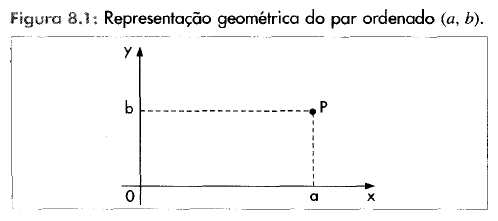
\includegraphics[height=5cm]{images/morettin_figura-8-1}
		\end{figure}
		
	\subsection{Relações em $\mathbb{R}^{2}$ \cite{morettin}}
	
		``Chama-se \textbf{relação binária}, ou simplesmente relação no $\mathbb{R}^{2}$, a todo conjunto de $\mathbb{R}^{2}$".

		\bigskip

		``\textbf{Exemplo 8.2}. Seja $A = \{(x, y) \in \mathbb{R}^{2} | y = 2x + 1 \}$. A representação geométrica do conjunto $A$ é uma reta"

		\begin{figure}[H]
			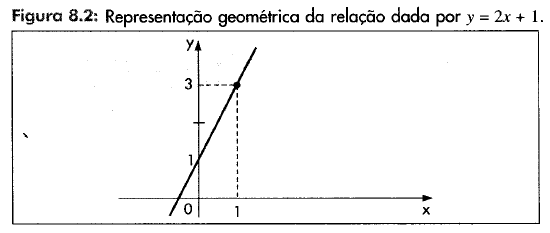
\includegraphics[height=5cm]{images/morettin_figura-8-2}
		\end{figure}

		``\textbf{Exemplo 8.3}. Considerando $C = \{(x, y) \in \mathbb{R}^{2} \ | \ x^{2} + y^{2} \leq 4\}$, a representação geométrica do conjunto $C$ é um círculo de centro na origem e raio $2$ (Figura 8.4)".

		\begin{figure}[H]
			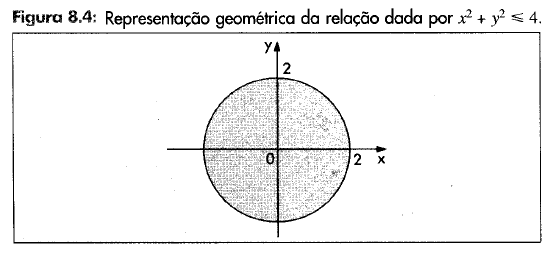
\includegraphics[height=5cm]{images/morettin_figura-8-4}
		\end{figure}

		\textbf{Observação}

		Lembremos que, se tivermos no plano cartesiano a representação gráfica de uma função $y = f(x)$, os pontos que estão ``acima" do gráfico satisfazem a relação $y > f(x)$.

		No caso de termos a representação geométrica de uma circunferência de equação $(x - a)^{2} + (y - b)^{2} = r^{2}$, de centro $C(a, b)$ e raio $r$, os pontos interiores a ela satisfazem a relação $(x - a)^{2} + (y - b)^{2} < r^{2}$, e os pontos exteriores a ela satisfazem a relação $(x - a)^{2} + (y - b)^{2} > r^{2}$.

		Uma relação do tipo $x  > k$ é representada geometricamente pelos pontos do plano à direita da reta vertical $x = k$; a relação $x < k$ é representada pelos pontos à esquerda da reta vertical $x = k$.

	\subsection{Equação do Círculo \cite{wikipedia}}

		Em um sistema cartesiano bidimensional $\mathbb{R}^{2}$, um círculo com as coordenadas de centro $(a, b)$ e raio $r$ se dá pelo conjunto de todos os pontos $(x, y)$ tal que

		\bigskip

		{\LARGE $(x - a)^{2} + (y - b)^{2} = r^{2}$} .

		\bigskip

		Esta equação, conhecida como a equação do círculo, segue o teorema de Pitágoras aplicado a qualquer ponto no círculo - como demonstrado no diagrama abaixo, o raio é a hipotenusa de um triângulo reto que tem como catetos $|x - a|$ e $|y - b|$. Se o círculo está centrado na origem $(0, 0)$, a equação se simplifica para

		\bigskip

		{\LARGE $x^{2} + y^{2} = r^{2}$} .

		\begin{figure}[H]
			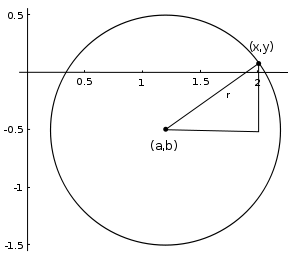
\includegraphics[height=5cm]{images/wikipedia_circle-equation}
		\end{figure}
		
	\subsection{Distância entre Dois Pontos em $\mathbb{R}^{2}$ \cite{morettin}}

		``Sejam $(x_{1}, y_{1})$ e $(x_{2}, y_{2})$ dois elementos de $\mathbb{R}^{2}$, representados geometricamente pelos pontos $P_{1}$ e $P_{2}$. A distância entre eles é o número

		\bigskip

		{\LARGE $d(P_{1}, P_{2}) = \sqrt{(x_{2} - x_{1})^{2} + (y_{2} - y_{1})^{2}}$} [Teorema de Pitágoras].

		\bigskip

		Notemos que a distância representa o comprimento do segmento $\overline{P_{1}P_{2}}$ na representação geométrica (Figura 8.7). Quando não houver possibilidade de confusão, a distância é indicada simplesmente por $d$".

		\begin{figure}[H]
			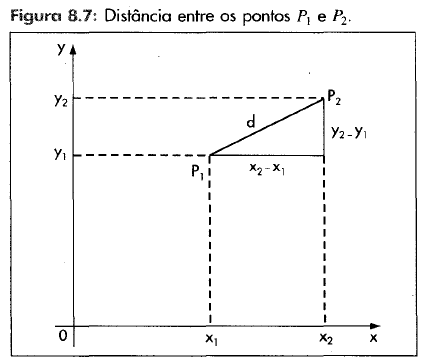
\includegraphics[height=7cm]{images/morettin_figura-8-7}
		\end{figure}

	\subsection{O Espaço Tridimensional \cite{morettin}}

		Seja $\mathbb{R}$ o conjunto dos números reais. O conjunto formado por todas as triplas ordenadas de reais é chamado \textbf{espaço tridimensional} e é indicado por $\mathbb{R} \times \mathbb{R} \times \mathbb{R}$ ou simplesmente $\mathbb{R}^{3}$. Assim:

		\bigskip

		{\LARGE $\mathbb{R}^{3} = \{(a, b, c) \ | \ a \in \mathbb{R}, \ b \in \mathbb{R}, \ c \in \mathbb{R} \}$} .
		
		\bigskip		
		
		Geometricamente, um elemento $(a, b, c)$ pode ser representado por um ponto $P$ de abscissa $a$, ordenada $b$ e cota $c$, num sistema de eixos $Ox$, $Oy$ e $Oz$ perpendiculares dois a dois. A cota $c$ é a distância do ponto $P$ em relação ao plano determinado pelos eixos $Ox$ e $Oy$, precedida pelo sinal $+$ se o ponto estiver "acima" do plano, e precedida pelo sinal $-$ se estiver "abaixo" desse plano (Figura 8.8).
		
		\begin{figure}[H]
			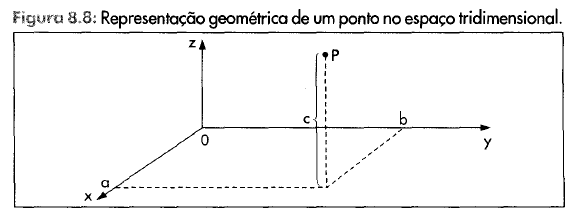
\includegraphics[height=5cm]{images/morettin_figura-8-8}
		\end{figure}

	\subsection{Relações em $\mathbb{R}^{3}$ \cite{morettin}}

		Chama-se relações no $\mathbb{R}^{3}$ a todo conjunto do $\mathbb{R}^{3}$.

		\bigskip

		\textbf{Exemplo 8.7}. Seja $A = \{(x, y, z) \ | \ x = 0 \}$, a representação geométrica de $A$ é o plano determinando pelos eixos $Oy$ e $Oz$ (Figura 8.9)

		\begin{figure}[H]
			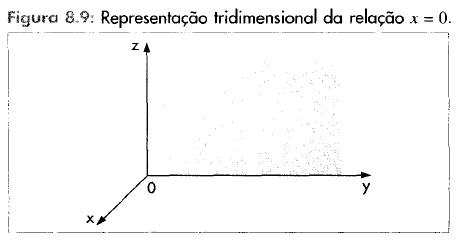
\includegraphics[height=5cm]{images/morettin_figura-8-9}
		\end{figure}

		\textbf{Exemplo 8.8}. Seja $B = \{(x, y, z) \ | \ z = 2 \}$, a representação geométrica desse conjunto é o plano paralelo determinando por $Ox$ e $Oy$ e distante duas unidades do mesmo (Figura 8.10)

		\begin{figure}[H]
			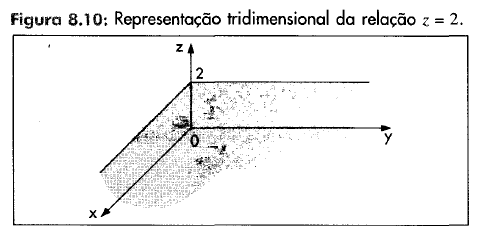
\includegraphics[height=5cm]{images/morettin_figura-8-10}
		\end{figure}

	\subsection{Equação do Plano em $\mathbb{R}^{3}$ \cite{morettin}}

		Pode se provar que toda relação do $\mathbb{R}^{3}$ que satisfaz uma equação do tipo $ax + bx + cz + d = 0$ (com $a, b, c, d$ reais e $a, b, c$ não nulos simultaneamente) tem por representação geométrica um plano no espaço tridimensional. O gráfico \textbf{por onde passa} tal plano pode ser obtido por meio de três pontos não alinhados.

		\begin{figure}[H]
			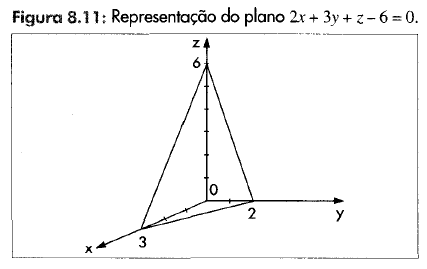
\includegraphics[height=6cm]{images/morettin_figura-8-11}
		\end{figure}

	\subsection{Distância entre Dois Pontos em $\mathbb{R}^{3}$ \cite{morettin}}

		Sejam $(x_{1}, y_{1}, z_{1})$ e $(x_{2}, y_{2}, z_{2})$ dois elementos de $\mathbb{R}^{3}$ representados pelos pontos $P_{1}$ e $P_{2}$. Chama-se a distância entre eles o número

		\bigskip

		{\LARGE $d(P_{1}, P_{2}) = \sqrt{(x_{2} - x_{1})^{2} + (y_{2} - y_{1})^{2} + (z_{2} - z_{1})^{2}}$}
		
		[Teorema de Pitágoras].

		\bigskip


		Dessa forma, a distância é o comprimento do segmento $\overline{P_{1}P_{2}}$ da Figura 8.12.

		\begin{figure}[H]
			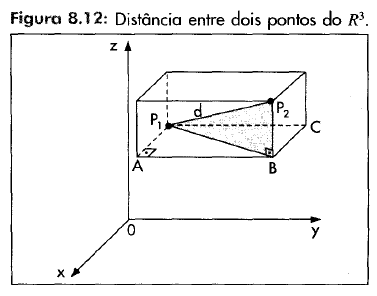
\includegraphics[height=7cm]{images/morettin_figura-8-12}
		\end{figure}

		\textbf{Dedução}

		Um dos catetos (altura) do triângulo $\overline{P_{1}BP_{2}}$ pode ser representado por $z_{2} - z_{1}$, já o outro cateto é a hipotenusa do triângulo $\overline{AP_{1}B}$ que é igual a $\sqrt{(x_{2} - x_{1})^{2} + (y_{2} - y_{1})^{2}}$. Logo temos que $d^{2} = (\sqrt{(x_{2} - x_{1})^{2} + (y_{2} - y_{1})^{2}})^{2} + (z_{2} - z_{1})^{2}$ o que simplificando fica $d(P_{1}, P_{2}) = \sqrt{(x_{2} - x_{1})^{2} + (y_{2} - y_{1})^{2} + (z_{2} - z_{1})^{2}}$.
		
	\subsection{O Conjunto $\mathbb{R}^{n}$ \cite{morettin}}

		Seja $\mathbb{R}$ o conjunto dos números reais. O conjunto formado pelas ênuplas ordenadas (sequências de $n$ elementos) de reais é chamado de espaço $n$-dimensional e é indicado por $\mathbb{R}^{n}$.

		Em particular, o conjunto $\mathbb{R}^{1}$ é o próprio conjunto dos números reais (representados geometricamente num único eixo). Os elementos de $\mathbb{R}^{n}$, pana $n > 3$, não admitem representação geométrica.

		Dado dois elementos do $\mathbb{R}^{n}$, $P_{1}(x_{1}, x_{2}, \dots , x_{n})$ e $P_{2}(y_{1}, y_{2}, \dots , y_{n})$ a distância entre eles é o número

		\bigskip

		{\LARGE $d(P_{1}, P_{2}) = \sqrt{(y_{1} - x_{1})^{2} + (y_{2} - x_{2})^{2} + \dots + (y_{n} - x_{n})^{2}}$}
		
		[Teorema de Pitágoras].
		
	\subsection{Bola Aberta \cite{morettin}}

		Seja $C$ um elemento do $R^{n}$ e $r$ um número real positivo. Chama-se bola aberta de centro $C$ e raio $r$ ao conjunto dos pontos do $R^{n}$ cuja distância até $C$ é menor que $r$. Isto é, a bola aberta é o conjunto

		\bigskip

		{\LARGE $B(C, r) = \{P \in R^{n} \mid d(P, C) < r\}$} .

		\bigskip

		\textbf{Exemplo 8.11}. A bola aberta do $\mathbb{R}^{2}$ de centro $C(4, 4)$ e raio $1$ é o interior do círculo representado na Figura 8.13.
		
		\begin{figure}[H]
			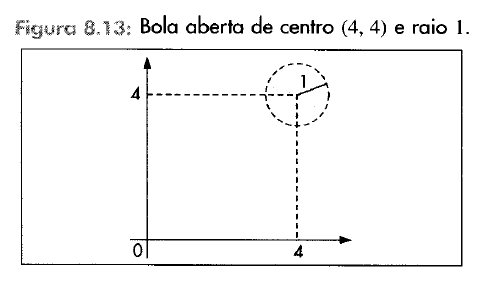
\includegraphics[height=6cm]{images/morettin_figura-8-13}
		\end{figure}

				\bigskip

		\textbf{Exemplo 8.12}. A bola aberta do $\mathbb{R}^{3}$ de centro $C(2, 3, 4)$ e raio $1$ é a região interior da esfera representada na Figura 8.14.
		
		\begin{figure}[H]
			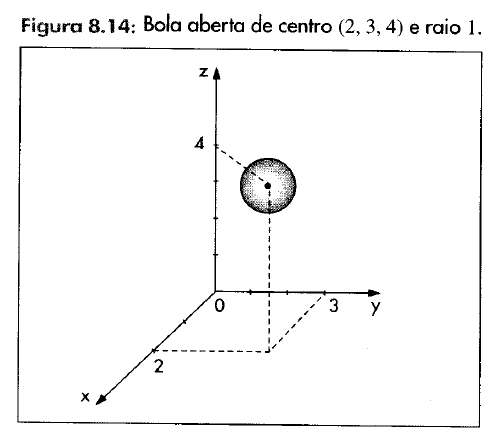
\includegraphics[height=7cm]{images/morettin_figura-8-14}
		\end{figure}
		
	\subsection{Ponto Interior \cite{morettin}}

		Seja $A$ um subconjunto do $R^{n}$; um elemento $P$ do $R^{n}$ é chamado ponto interior de $A$ se existir uma bola aberta com centro em $P$ contida em $A$. Isto é, $P$ é um ponto interior de $A$ se exisitir um real $r > 0$, tal que $B(P, r) \subset A$.

		\bigskip

		\textbf{Exemplo 8.13}. Seja $A = \{(x, y) \in \mathbb{R}^2 \mid y \geq 2\}$. O ponto $P(4, 4)$ é interior a $A$ e o ponto $P(3, 2)$ não é interior a $A$ (Figura 8.15).

		\begin{figure}[H]
			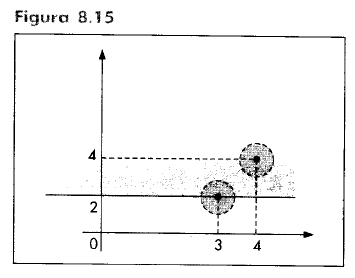
\includegraphics[height=6cm]{images/morettin_figura-8-15}
		\end{figure}
		
	\subsection{Conjunto Aberto \cite{morettin}}

		Seja $A$ um subconjunto do $\mathbb{R}^{n}$. $A$ é chamado de conjunto aberto se todos os seus pontos são interiores.

		\textbf{Exemplo 8.14}. O conjunto $A = \{(x, y) \in \mathbb{R}^2 \mid x > 2\}$ é aberto, pois todos os seus pontos são interiores (Figura 8.16).

		\begin{figure}[H]
			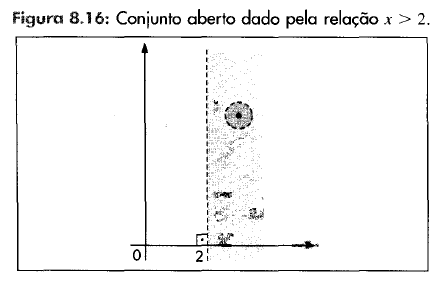
\includegraphics[height=6.5cm]{images/morettin_figura-8-16}
		\end{figure}

	\subsection{Pontos de Fronteira de um Conjunto \cite{morettin}}

		Seja $A$ um subconjunto do $\mathbb{R}^{n}$. Um ponto de $A$ que não é interior chama-se ponto de fronteira de $A$.

		\textbf{Exemplo 8.16}. Seja $A = \{(x, y) \in \mathbb{R}^2 \mid y \geq 2\}$. Os pontos da reta $y = 2$ são pontos de fronteira de $A$ (Figura 8.18).

		\begin{figure}[H]
			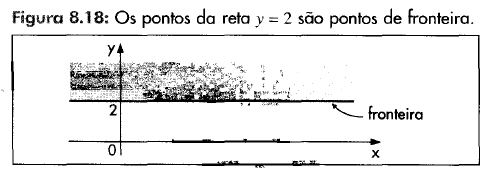
\includegraphics[height=3.5cm]{images/morettin_figura-8-18}
		\end{figure}
		
	\subsection{Planos Coordenados \cite{google}}

		Os três eixos coordenados $Ox$, $Oy$ e $Oz$ definem três planos perpendiculares entre si. Em $xOy$ temos z como constante (em que $O$ é o ponto $(0, 0, z_{0})$); em $yOz$ temos x como constante (em que $O$ é o ponto $(x_{0}, 0, 0)$); e em $xOz$ temos y como constante (em que $O$ é o ponto $(0, y_{0}, 0)$).

		\begin{figure}[H]
			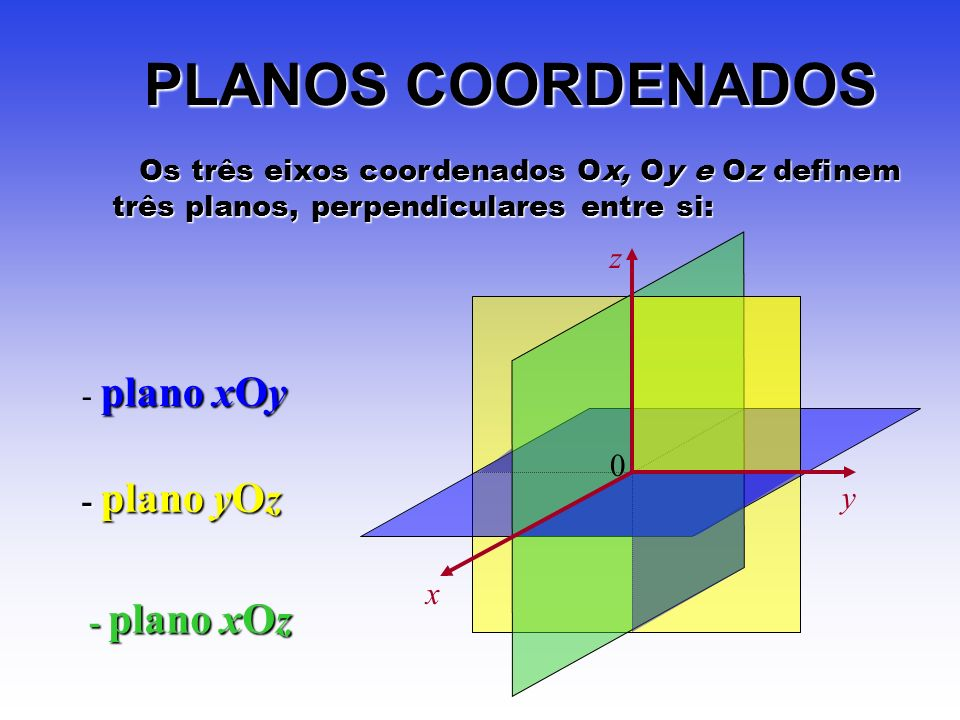
\includegraphics[height=8cm]{images/google-images_planos-coordenados}
		\end{figure}
		
		Uma das formas de criar um gráfico de um função em $\mathbb{R}^{3}$ é desenhar o cruzamento dos gráficos das funções em $xOz$ e $yOz$. Exemplo:
		
		\begin{figure}[H]
			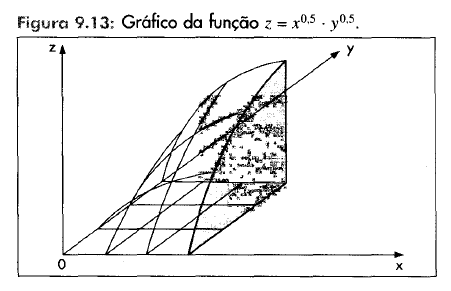
\includegraphics[height=6cm]{images/morettin_figura-9-13}
		\end{figure}